\documentclass[aspectratio=169, 11pt]{beamer}

% === Theme ===
\usetheme{Madrid}
\usecolortheme{whale}
\setbeamertemplate{navigation symbols}{}
\setbeamertemplate{footline}[frame number]

% === Packages ===
\usepackage[utf8]{inputenc}
\usepackage[vietnamese]{babel}
\usepackage{graphicx}
\usepackage{booktabs}
\usepackage{amsmath}
\usepackage{listings}
\usepackage{xcolor}
\usepackage{hyperref}

% === Code style ===
\lstset{
  basicstyle=\ttfamily\small,
  keywordstyle=\color{blue}\bfseries,
  commentstyle=\color{gray},
  stringstyle=\color{red},
  breaklines=true,
  frame=single,
  backgroundcolor=\color{gray!10},
}

% === Title ===
\title[Session-based RS]{Chủ Đề 9: Hệ Thống Khuyến Nghị\\Dựa Trên Hành Vi Duyệt Web}
\subtitle{Session-based Recommendation System}
\author[Phương, Hoàng, Nam]{Phan Nguyễn Mai Phương -- 25002711\\Ngô Quốc Hoàng -- 25001771\\Bùi Thức Nam -- 25003881}
\institute{Trường Đại học Công nghiệp TP.HCM\\Khoa Công nghệ Thông tin\\GVHD: TS. Lê Thị Vĩnh Thanh}
\date{2024--2025}

\begin{document}

% ============================================================
% SLIDE 1: TRANG BÌA
% ============================================================
\begin{frame}
\titlepage
\end{frame}

% ============================================================
% SLIDE 2: NỘI DUNG TRÌNH BÀY
% ============================================================
\begin{frame}{Nội dung trình bày}
\tableofcontents
\end{frame}

% ============================================================
% PHẦN 1: GIỚI THIỆU BÀI TOÁN
% ============================================================
\section{Giới thiệu bài toán}

\begin{frame}{Bài toán thực tế}
\begin{columns}
\begin{column}{0.55\textwidth}
\textbf{Tình huống:}
\begin{itemize}
    \item Khách hàng \textbf{ẩn danh} truy cập website bán hàng
    \item Không đăng nhập, không có tài khoản
    \item Trong 10 phút, click xem lần lượt:
\end{itemize}

\vspace{0.3cm}
\centering
\fbox{Áo thun} $\longrightarrow$ \fbox{Quần jean} $\longrightarrow$ \fbox{Giày} $\longrightarrow$ \colorbox{red!20}{\textbf{???}}

\vspace{0.3cm}
\textbf{Câu hỏi:} Gợi ý sản phẩm nào tiếp theo?
\end{column}

\begin{column}{0.4\textwidth}
\begin{block}{Ứng dụng thực tế}
\begin{itemize}
    \item Amazon (khách vãng lai)
    \item Shopee, Tiki
    \item Trang tin tức
    \item Streaming video
\end{itemize}
\end{block}
\end{column}
\end{columns}
\end{frame}

\begin{frame}{Định nghĩa hình thức}
\begin{block}{Session-based Recommendation}
Cho một phiên (session) $S = [i_1, i_2, \ldots, i_t]$ là chuỗi sản phẩm người dùng đã tương tác theo thứ tự thời gian.

\vspace{0.3cm}
\textbf{Mục tiêu:} Dự đoán sản phẩm $i_{t+1}$ mà người dùng sẽ tương tác tiếp theo.
\end{block}

\vspace{0.5cm}
\begin{center}
\begin{tabular}{ll}
\textbf{Input:} & Chuỗi $[i_1, i_2, \ldots, i_t]$ (các item đã click) \\
\textbf{Output:} & Top-K item có khả năng được click tiếp theo \\
\textbf{Đặc điểm:} & Không cần User ID, không cần lịch sử cũ \\
\end{tabular}
\end{center}
\end{frame}

\begin{frame}{So sánh với Collaborative Filtering}
\begin{table}
\centering
\begin{tabular}{lcc}
\toprule
\textbf{Tiêu chí} & \textbf{CF truyền thống} & \textbf{Session-based RS} \\
\midrule
Cần ID người dùng? & Bắt buộc & \textcolor{green!60!black}{\textbf{Không cần}} \\
Dùng lịch sử dài hạn? & Có (toàn bộ) & \textcolor{green!60!black}{\textbf{Không}} \\
Cold-start user mới? & Không giải quyết & \textcolor{green!60!black}{\textbf{Xử lý được}} \\
Sở thích tức thời? & Kém & \textcolor{green!60!black}{\textbf{Tốt}} \\
\midrule
Ứng dụng & Netflix, Spotify & Amazon, Shopee \\
\bottomrule
\end{tabular}
\end{table}

\vspace{0.3cm}
\begin{alertblock}{Kết luận}
Session-based RS phù hợp khi: người dùng ẩn danh, phiên ngắn, cần gợi ý real-time.
\end{alertblock}
\end{frame}

% ============================================================
% PHẦN 2: DỮ LIỆU
% ============================================================
\section{Dữ liệu và tiền xử lý}

\begin{frame}{Cấu trúc dữ liệu Session}
\begin{table}
\centering
\small
\begin{tabular}{ccccc}
\toprule
\textbf{SessionID} & \textbf{Timestamp} & \textbf{ItemID} & \textbf{Action} \\
\midrule
S001 & 09:01:03 & I042 & click \\
S001 & 09:03:45 & I087 & click \\
S001 & 09:07:12 & I015 & click \\
S001 & 09:09:55 & I033 & click \\
\midrule
S002 & 10:15:00 & I201 & click \\
S002 & 10:18:30 & I202 & click \\
\bottomrule
\end{tabular}
\end{table}

\vspace{0.3cm}
\begin{itemize}
    \item Phiên S001 $\rightarrow$ chuỗi: $[\text{I042}, \text{I087}, \text{I015}, \text{I033}]$
    \item Phiên S002 $\rightarrow$ chuỗi: $[\text{I201}, \text{I202}]$
    \item Mỗi phiên là một ``câu chuyện'' \textbf{độc lập}
\end{itemize}
\end{frame}

\begin{frame}{Dataset: Yoochoose (RecSys Challenge 2015)}
\begin{columns}
\begin{column}{0.5\textwidth}
\begin{table}
\centering
\small
\begin{tabular}{ll}
\toprule
\textbf{Thuộc tính} & \textbf{Giá trị} \\
\midrule
Tổng click & 33 triệu \\
Số phiên & 9.2 triệu \\
Số sản phẩm & 52,739 \\
Lĩnh vực & E-commerce \\
\midrule
\multicolumn{2}{c}{\textit{Sau lấy mẫu 1/64:}} \\
\midrule
Số phiên (mẫu) & 144,527 \\
Sau lọc & 116,267 \\
Train & 108,263 \\
Test & 8,004 \\
\bottomrule
\end{tabular}
\end{table}
\end{column}

\begin{column}{0.45\textwidth}
\begin{block}{Tiền xử lý}
\begin{enumerate}
    \item Chia train/test theo \textbf{thời gian} (90/10)
    \item Lọc item hiếm ($<5$ lần, \textbf{chỉ trên train})
    \item Lọc độ dài phiên $\in [2,20]$
\end{enumerate}
\end{block}

\vspace{0.3cm}
\begin{alertblock}{Lưu ý}
Chia theo thời gian TRƯỚC, rồi lọc item hiếm chỉ trên train $\rightarrow$ tránh data leakage.
\end{alertblock}
\end{column}
\end{columns}
\end{frame}

% ============================================================
% PHẦN 3: THUẬT TOÁN SKNN
% ============================================================
\section{Thuật toán SKNN}

\begin{frame}{SKNN -- Ý tưởng}
\begin{block}{Session K-Nearest Neighbors (SKNN)}
Tìm $K$ phiên lịch sử \textbf{tương tự nhất} với phiên hiện tại, sau đó tổng hợp các item từ những phiên đó để sinh khuyến nghị.
\end{block}

\vspace{0.4cm}
\textbf{Ký hiệu:}
\begin{table}
\centering
\small
\begin{tabular}{ll}
$S_q = [i_1, i_2, \ldots, i_t]$ & phiên truy vấn (phiên hiện tại) \\
$\mathcal{S} = \{S_1, S_2, \ldots, S_N\}$ & tập tất cả phiên lịch sử \\
$K$ & số hàng xóm gần nhất (hyperparameter) \\
$\text{KNN}(S_q)$ & $K$ phiên có similarity cao nhất với $S_q$ \\
\end{tabular}
\end{table}
\end{frame}

\begin{frame}{SKNN -- Công thức}
\textbf{1. Đo độ tương tự giữa hai phiên:}
\begin{equation}
\text{sim}(S_q, S_n) = \frac{|S_q \cap S_n|}{\sqrt{|S_q| \times |S_n|}}
\end{equation}
\small
$|S_q \cap S_n|$: số item trùng nhau. \quad Giá trị $\in [0, 1]$.

\vspace{0.4cm}
\normalsize
\textbf{2. Tính điểm cho item ứng viên $i$ ($i \notin S_q$):}
\begin{equation}
\text{score}(i) = \sum_{S_n \in \text{KNN}(S_q)} \text{sim}(S_q, S_n) \times \mathbb{1}[i \in S_n]
\end{equation}
\small
$\mathbb{1}[i \in S_n] = 1$ nếu item $i$ có trong phiên $S_n$, ngược lại $= 0$.

\vspace{0.4cm}
\normalsize
\textbf{3. Sinh khuyến nghị:}
\begin{equation}
\text{Top-N} = \underset{i \notin S_q}{\text{argmax-N}} \; \text{score}(i)
\end{equation}
\end{frame}

\begin{frame}[fragile]{SKNN -- Mã giả thuật toán}
\begin{block}{Algorithm 1: SKNN Prediction}
\begin{verbatim}
Input:  Sq (current session), S (history sessions), K, N
Output: Top-N recommended items

1:  for each Sn in S do
2:      sim(Sq,Sn) = |Sq INTERSECT Sn| / sqrt(|Sq|*|Sn|)
3:  end for
4:  sort S by sim (descending)
5:  KNN <- top-K sessions with sim > 0
6:  for each item i in KNN with i NOT IN Sq do
7:      score(i) = SUM( sim(Sq,Sn) * 1[i in Sn] )
8:  end for
9:  sort items by score (descending)
10: return Top-N items
\end{verbatim}
\end{block}
\small
\textbf{Complexity:} $O(|\mathcal{S}| \times |S_q|)$ -- dùng inverted index để tăng tốc.
\end{frame}

\begin{frame}{SKNN -- Ví dụ tính tay}
\small
\textbf{Cho:} $S_q = \{I1, I2, I3\}$, \; $K = 3$

\vspace{0.2cm}
\textbf{Bước 1 -- Tính similarity:}
\begin{table}
\centering
\footnotesize
\begin{tabular}{lccc}
\toprule
\textbf{Phiên} & \textbf{Giao với $S_q$} & \textbf{Công thức} & \textbf{sim} \\
\midrule
$S_1 = \{I1, I2, I3, I4\}$ & $\{I1, I2, I3\}$ & $3/\sqrt{3 \times 4}$ & $\mathbf{0.866}$ \\
$S_2 = \{I1, I2, I5\}$ & $\{I1, I2\}$ & $2/\sqrt{3 \times 3}$ & $0.667$ \\
$S_3 = \{I2, I3, I6\}$ & $\{I2, I3\}$ & $2/\sqrt{3 \times 3}$ & $0.667$ \\
$S_4 = \{I5, I6, I7\}$ & $\emptyset$ & -- & $0.000$ \\
\bottomrule
\end{tabular}
\end{table}

\textbf{Bước 2 -- KNN:} $\{S_1, S_2, S_3\}$

\vspace{0.1cm}
\textbf{Bước 3 -- Score} (loại $\{I1, I2, I3\}$):
\footnotesize
\begin{itemize}
    \item $\text{score}(I4) = 0.866 \times 1 + 0.667 \times 0 + 0.667 \times 0 = \mathbf{0.866}$
    \item $\text{score}(I5) = 0 + 0.667 \times 1 + 0 = 0.667$
    \item $\text{score}(I6) = 0 + 0 + 0.667 \times 1 = 0.667$
\end{itemize}

\small
\textbf{Bước 4 -- Khuyến nghị:} $[I4, I5, I6]$ \; $\checkmark$
\end{frame}

% ============================================================
% PHẦN 4: THUẬT TOÁN GRU4Rec
% ============================================================
\section{Thuật toán GRU4Rec}

\begin{frame}{GRU4Rec -- Tổng quan}
\begin{block}{Ý tưởng chính (Hidasi et al., ICLR 2016)}
Dùng mạng hồi quy GRU để học biểu diễn ẩn của chuỗi hành vi, từ đó dự đoán item tiếp theo.
\end{block}

\vspace{0.3cm}
\textbf{Ký hiệu:}
\begin{table}
\centering
\small
\begin{tabular}{ll}
$M$ & tổng số item trong catalog \\
$E \in \mathbb{R}^{M \times d}$ & ma trận embedding (d = 64) \\
$e_{i_t} = E[i_t]$ & vector embedding của item $i_t$ \\
$h_t \in \mathbb{R}^{H}$ & hidden state tại bước $t$ (H = 128) \\
$W_o \in \mathbb{R}^{H \times M}$ & ma trận output \\
\end{tabular}
\end{table}

\vspace{0.3cm}
\textbf{Pipeline:}
$$i_t \xrightarrow{\text{Embed}} e_{i_t} \xrightarrow{\text{GRU}} h_t \xrightarrow{\text{Linear}} \hat{y}_t \in \mathbb{R}^M \xrightarrow{\text{softmax}} P(i_{t+1})$$
\end{frame}

\begin{frame}{GRU -- Công thức chi tiết}
Tại mỗi bước $t$, nhận input $x_t = e_{i_t}$ và hidden state $h_{t-1}$:

\begin{align}
z_t &= \sigma(W_z x_t + U_z h_{t-1} + b_z) & \text{(Update gate)} \\
r_t &= \sigma(W_r x_t + U_r h_{t-1} + b_r) & \text{(Reset gate)} \\
\tilde{h}_t &= \tanh(W_h x_t + U_h (r_t \odot h_{t-1}) + b_h) & \text{(Candidate)} \\
h_t &= (1 - z_t) \odot h_{t-1} + z_t \odot \tilde{h}_t & \text{(New state)}
\end{align}

\vspace{0.3cm}
\begin{table}
\centering
\small
\begin{tabular}{ll}
\toprule
\textbf{Ký hiệu} & \textbf{Ý nghĩa} \\
\midrule
$z_t \approx 0$ & Giữ nguyên $h_{t-1}$ (nhớ quá khứ) \\
$z_t \approx 1$ & Thay bằng $\tilde{h}_t$ (học từ hiện tại) \\
$r_t$ & Kiểm soát quá khứ ảnh hưởng đến candidate \\
$\odot$ & Phép nhân element-wise \\
\bottomrule
\end{tabular}
\end{table}
\end{frame}

\begin{frame}{GRU4Rec -- Scoring}
Sau khi GRU xử lý chuỗi, lấy hidden state cuối $h_t$:

\vspace{0.3cm}
\textbf{Logits:}
\begin{equation}
\hat{y}_t = W_o \cdot h_t + b_o \in \mathbb{R}^M
\end{equation}

\textbf{Xác suất (softmax):}
\begin{equation}
P(i_{t+1} = j \;|\; S_{1:t}) = \frac{\exp(\hat{y}_t[j])}{\sum_{k=1}^{M} \exp(\hat{y}_t[k])}
\end{equation}

\textbf{Khuyến nghị:} Lấy Top-N item có $\hat{y}_t[j]$ cao nhất (loại item đã xem).
\end{frame}

\begin{frame}{GRU4Rec -- Loss Function}
\textbf{Cross-Entropy Loss:}
\begin{equation}
\mathcal{L}_{CE} = -\frac{1}{|\mathcal{D}|} \sum_{(S, i^+) \in \mathcal{D}} \log P(i^+ | S)
\end{equation}
\small $i^+$: item thực sự được click tiếp theo (ground truth).

\vspace{0.5cm}
\normalsize
\textbf{BPR Loss} (Bayesian Personalized Ranking):
\begin{equation}
\mathcal{L}_{BPR} = -\frac{1}{|\mathcal{D}|} \sum_{(S, i^+)} \frac{1}{N_s}\sum_{j=1}^{N_s} \log \sigma(\hat{y}[i^+] - \hat{y}[j])
\end{equation}
\small $j$: negative sample (item ngẫu nhiên), $\sigma$: sigmoid.

\vspace{0.3cm}
\normalsize
\begin{alertblock}{Mục tiêu}
Đảm bảo score item đúng ($i^+$) luôn cao hơn item sai ($j$).
\end{alertblock}
\end{frame}

\begin{frame}[fragile]{GRU4Rec -- Mã giả thuật toán}
\begin{block}{Algorithm 2: GRU4Rec Training}
\begin{verbatim}
Input:  sessions S, learning rate eta, epochs E
Output: model parameters theta

1:  initialize theta ~ N(0, 0.01)
2:  for epoch = 1 to E do
3:    for each mini-batch B in S do
4:      for each session [i1,...,iT] in B do
5:        h0 <- 0
6:        for t = 1 to T-1 do
7:          et <- E[it]           // embedding
8:          ht <- GRU(et, h(t-1)) // forward
9:          yt <- Wo*ht + bo      // logits
10:         Lt <- -log P(i(t+1)|yt)
11:       end for
12:     end for
13:     theta <- theta - eta * grad(L)
14:   end for
15: end for
\end{verbatim}
\end{block}
\end{frame}

\begin{frame}[fragile]{GRU4Rec -- Mã giả Prediction}
\begin{block}{Algorithm 3: GRU4Rec Inference}
\begin{verbatim}
Input:  Sq = [i1,...,it], trained model, Top-N
Output: N item khuyen nghi

1:  h0 <- 0
2:  for k = 1 to t do
3:    ek <- E[ik]           // embedding lookup
4:    hk <- GRU(ek, h(k-1)) // forward GRU
5:  end for
6:  y <- Wo * ht + bo       // score moi item
7:  y[i] <- -inf, for all i in Sq  // loai da xem
8:  return Top-N item co y[j] cao nhat
\end{verbatim}
\end{block}

\vspace{0.2cm}
\textbf{Complexity:}
\begin{itemize}
    \item Training: $O(E \times |\mathcal{S}| \times \bar{T} \times (d \cdot H + H \cdot M))$
    \item Inference: $O(t \times d \cdot H + H \times M)$ -- \textbf{real-time}
\end{itemize}
\end{frame}

% ============================================================
% PHẦN 5: KẾT QUẢ THÍ NGHIỆM
% ============================================================
\section{Kết quả thí nghiệm}

\begin{frame}{Metrics đánh giá}
\begin{table}
\centering
\begin{tabular}{lll}
\toprule
\textbf{Chỉ số} & \textbf{Công thức} & \textbf{Ý nghĩa} \\
\midrule
Recall@20 & $\frac{|\text{hit}|}{|\text{test}|}$ & Tỉ lệ phiên có item đúng trong Top-20 \\[0.3cm]
MRR@20 & $\frac{1}{N}\sum \frac{1}{\text{rank}_i}$ & Trung bình nghịch đảo vị trí item đúng \\
\bottomrule
\end{tabular}
\end{table}

\vspace{0.5cm}
\begin{block}{Chiến lược đánh giá: Leave-one-out}
\begin{itemize}
    \item Phiên test: $[A, B, C, D]$
    \item Input cho mô hình: $[A, B, C]$
    \item Đáp án: $D$
    \item Kiểm tra: $D$ có nằm trong Top-20 gợi ý không?
\end{itemize}
\end{block}
\end{frame}

\begin{frame}{Kết quả trên Yoochoose (1/64)}
\begin{table}
\centering
\large
\begin{tabular}{lcc}
\toprule
\textbf{Mô hình} & \textbf{Recall@20} & \textbf{MRR@20} \\
\midrule
Popularity Baseline & 0.0187 (1.87\%) & 0.0041 \\
\textbf{SKNN (k=500)} & \textbf{0.2952 (29.5\%)} & \textbf{0.1349} \\
GRU4Rec (10 epoch) & 0.2796 (28.0\%) & 0.1262 \\
\bottomrule
\end{tabular}
\end{table}

\vspace{0.5cm}
\begin{columns}
\begin{column}{0.5\textwidth}
\begin{exampleblock}{Nhận xét}
\begin{itemize}
    \item SKNN vượt Popularity \textbf{+27.65 điểm}
    \item SKNN nhỉnh hơn GRU4Rec \textbf{+1.56 điểm}
    \item Cả hai đều vượt xa baseline
\end{itemize}
\end{exampleblock}
\end{column}
\begin{column}{0.45\textwidth}
\begin{alertblock}{Ý nghĩa}
Tận dụng thông tin chuỗi trong session thực sự có giá trị lớn so với chỉ dùng popularity.
\end{alertblock}
\end{column}
\end{columns}
\end{frame}

\begin{frame}{Biểu đồ so sánh}
\begin{center}
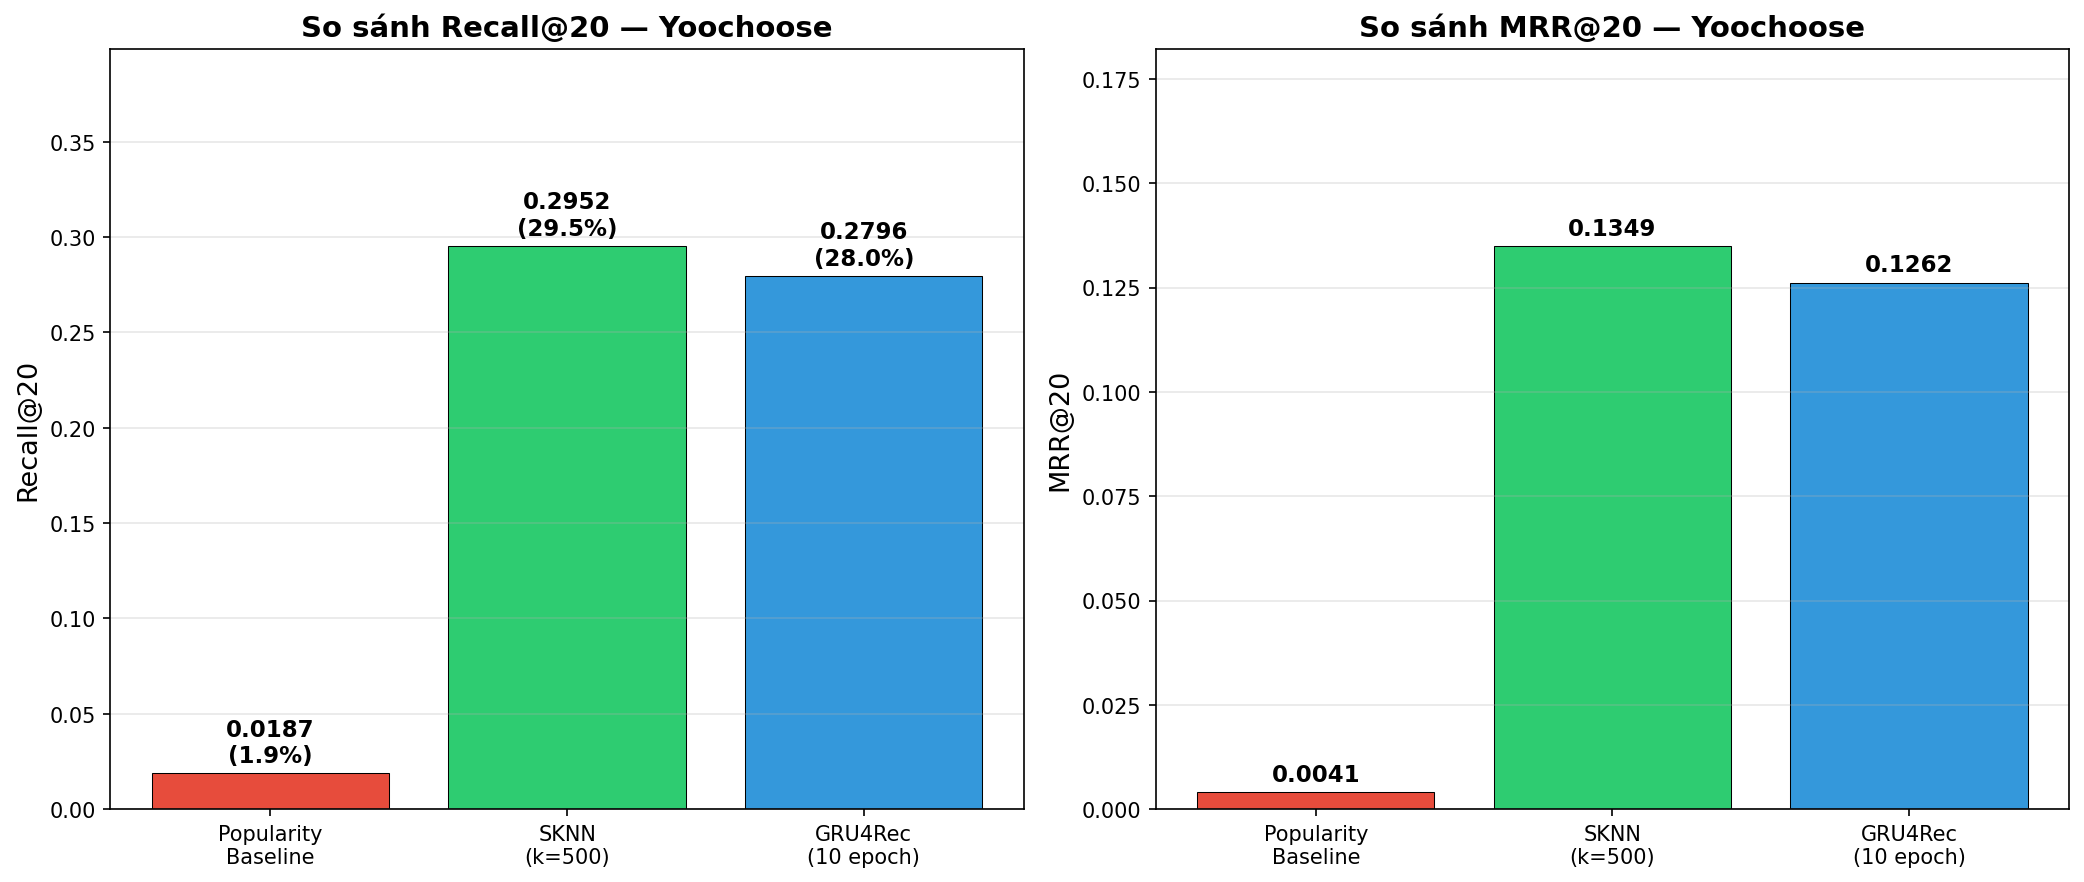
\includegraphics[width=0.85\textwidth]{../output/so_sanh_final.png}
\end{center}
\end{frame}

\begin{frame}{Ảnh hưởng của K (SKNN)}
\begin{columns}
\begin{column}{0.55\textwidth}
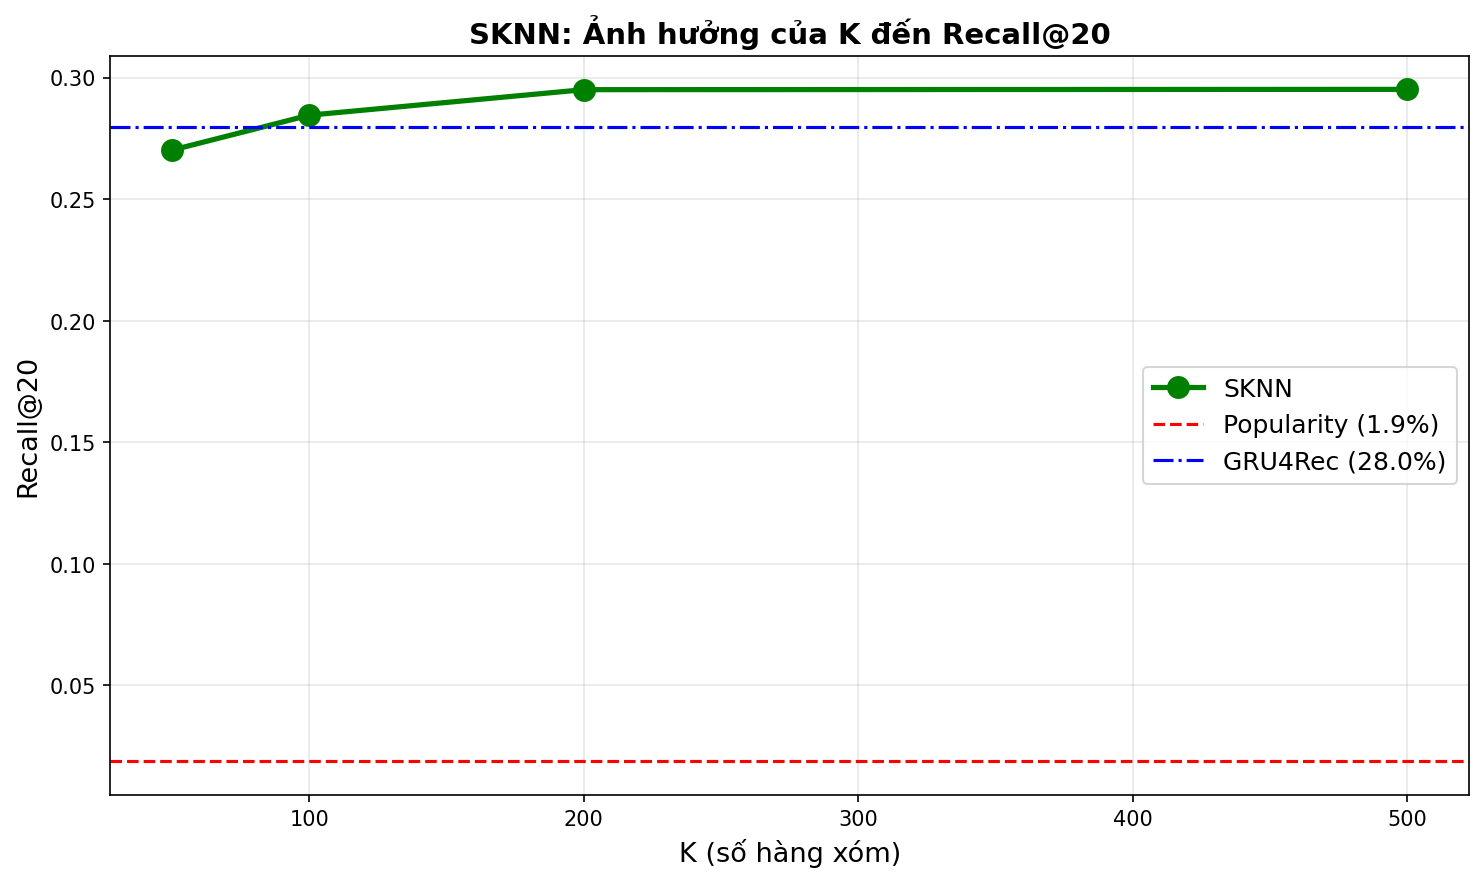
\includegraphics[width=\textwidth]{../output/recall_theo_k_final.png}
\end{column}
\begin{column}{0.4\textwidth}
\begin{itemize}
    \item K nhỏ (50): ít hàng xóm $\rightarrow$ bỏ sót item tốt
    \item K lớn: Recall tăng dần rồi \textbf{bão hòa} (200$\rightarrow$500 gần như không đổi)
    \item \textbf{K=500}: tốt nhất trong dải đã thử
\end{itemize}

\vspace{0.3cm}
\begin{table}
\centering
\small
\begin{tabular}{cc}
\toprule
K & Recall@20 \\
\midrule
50 & 0.2702 \\
100 & 0.2846 \\
200 & 0.2951 \\
\textbf{500} & \textbf{0.2952} \\
\bottomrule
\end{tabular}
\end{table}
\end{column}
\end{columns}
\end{frame}

\begin{frame}{GRU4Rec -- Training Loss}
\begin{columns}
\begin{column}{0.55\textwidth}
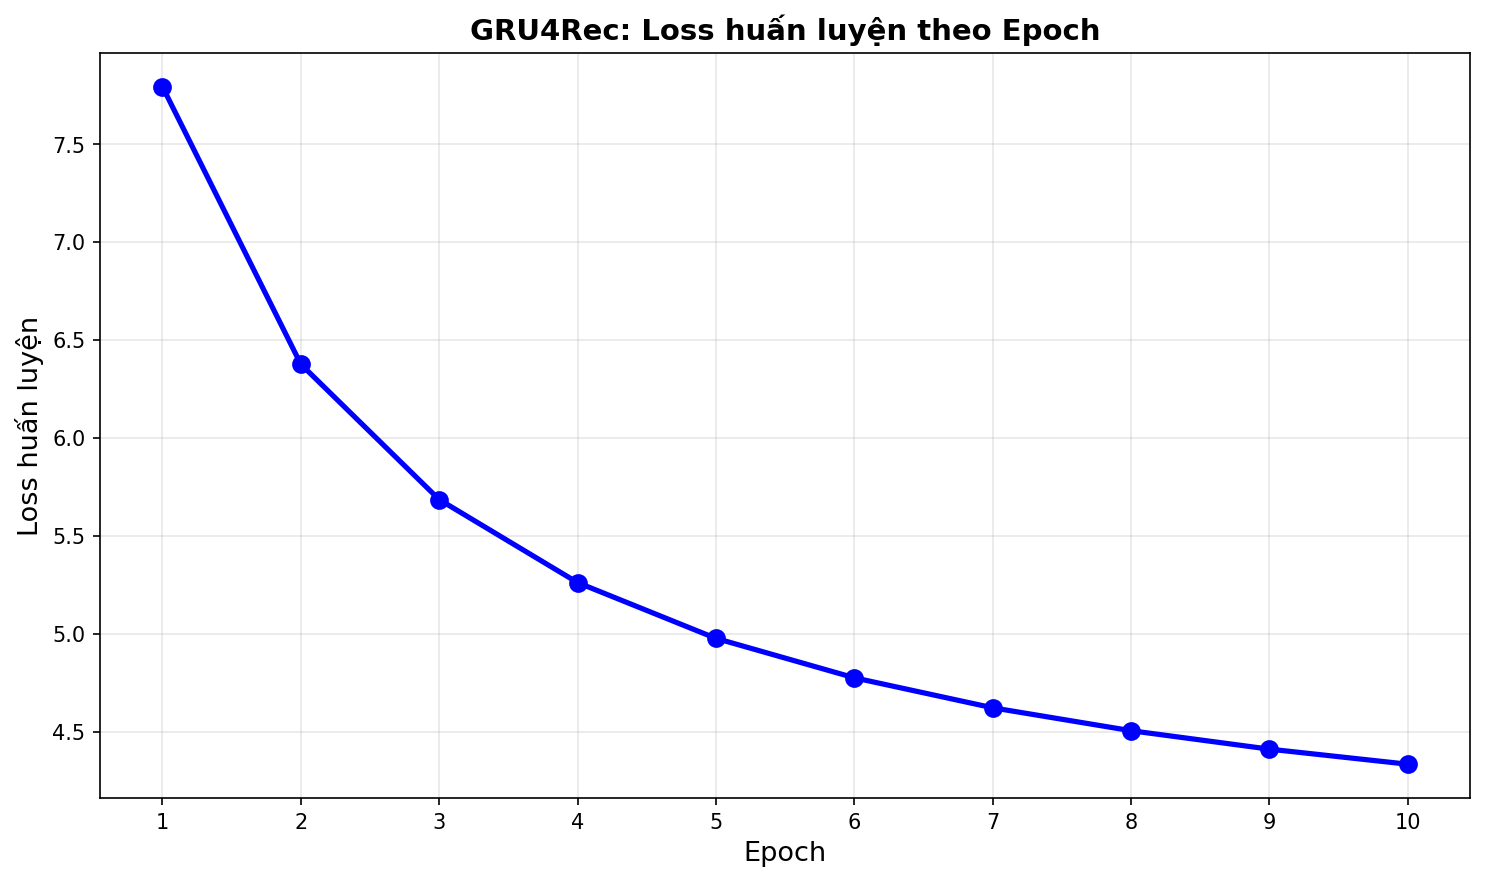
\includegraphics[width=\textwidth]{../output/gru4rec_loss_curve.png}
\end{column}
\begin{column}{0.4\textwidth}
\begin{itemize}
    \item Loss giảm đều qua 10 epoch
    \item Chưa hội tụ hoàn toàn
    \item Có thể cải thiện thêm với:
    \begin{itemize}
        \item Nhiều epoch hơn (20--30)
        \item Learning rate scheduling
        \item Larger hidden size
    \end{itemize}
\end{itemize}

\vspace{0.3cm}
\begin{block}{Cấu hình}
\small
Embedding: 64, Hidden: 128\\
Optimizer: Adam, lr=0.001\\
Batch size: 256
\end{block}
\end{column}
\end{columns}
\end{frame}

% ============================================================
% PHẦN 6: KẾT LUẬN
% ============================================================
\section{Kết luận}

\begin{frame}{Tổng kết}
\begin{table}
\centering
\begin{tabular}{lp{8cm}}
\toprule
\textbf{Nội dung} & \textbf{Điểm chính} \\
\midrule
Bài toán & Dự đoán item tiếp theo từ chuỗi hành vi phiên hiện tại \\
Khác CF & Không cần User ID, phù hợp phiên ẩn danh/cold-start user \\
SKNN & Đơn giản, hiệu quả, không cần GPU \\
GRU4Rec & Học được thứ tự click; cần thêm dữ liệu/epoch để cải thiện \\
Kết quả & Popularity 1.87\% $\rightarrow$ GRU4Rec 28.0\% $\rightarrow$ SKNN 29.5\% \\
\bottomrule
\end{tabular}
\end{table}

\vspace{0.5cm}
\begin{block}{Bài học thực nghiệm}
Nên bắt đầu với Popularity Baseline và SKNN. Nếu SKNN chưa vượt rõ Popularity, cần kiểm tra lại dữ liệu và protocol trước khi đầu tư vào mô hình học sâu.
\end{block}
\end{frame}

\begin{frame}{Hướng mở rộng}
\begin{table}
\centering
\begin{tabular}{lll}
\toprule
\textbf{Hướng} & \textbf{Mô tả} & \textbf{Độ khó} \\
\midrule
NARM & Thêm Attention vào GRU & $\star\star\star$ \\
SR-GNN & Session dạng đồ thị + GNN & $\star\star\star\star$ \\
BERT4Rec & BERT bidirectional cho session & $\star\star\star\star$ \\
Tiếng Việt & Dataset từ Tiki/Shopee & $\star\star\star$ \\
\bottomrule
\end{tabular}
\end{table}
\end{frame}

\begin{frame}{Tài liệu tham khảo}
\small
\begin{enumerate}
    \item Hidasi B. et al. (2016). \textit{Session-based Recommendations with Recurrent Neural Networks}. ICLR.\\
    \url{https://arxiv.org/abs/1511.06939}
    
    \item Ludewig M., Jannach D. (2018). \textit{Evaluation of Session-based Recommendation Algorithms}. UMUAI.\\
    \url{https://arxiv.org/abs/1803.09587}
    
    \item Jannach D. et al. (2017). \textit{When RNNs meet the Neighborhood for Session-Based Recommendation}. RecSys.
    
    \item Li J. et al. (2017). \textit{Neural Attentive Session-based Recommendation}. CIKM.
    
    \item Dataset: Yoochoose -- RecSys Challenge 2015.\\
    \url{https://www.kaggle.com/datasets/chadgostopp/recsys-challenge-2015}
\end{enumerate}
\end{frame}

% ============================================================
% SLIDE CUỐI
% ============================================================
\begin{frame}
\centering
\Huge\textbf{Cảm ơn thầy/cô đã lắng nghe!}

\vspace{1cm}
\Large Q \& A
\end{frame}

\end{document}
